\section{Differentialgleichungen}

\begin{definition}{Differentialgleichung n-ter Ordnung} 
ist eine Gleichung, in der Ableitungen einer unbekannten Funktion $y = y(x)$ bis zur $n$-ten Ordnung auftreten. Explizite Form:
\vspace{-2mm}\\
$$y^{(n)}(x) = f(x, y(x), y'(x), ..., y^{(n-1)}(x))$$
Gesucht sind die Lösungen $y = y(x)$ dieser Gleichung, wobei die Lösungen $y$ auf einem Intervall $[a,b]$ definiert sein sollen.

Implizite Form: nicht nach $y^{(n)}$ aufgelöst, sondern in Form \\ $F(x,y,y',y'',\ldots,y^{(n)})=0$ gegeben.
\end{definition}

\begin{concept}{Arten von DGL}
  \begin{itemize}
    \item \emph{Separierbar:} $y'=g(x)\cdot h(y)$\\
    $\rightarrow$ \(F(x,y)\) kann als Produkt eines \(x\)- \& \(y\)-Anteils geschrieben werden
      
    \item \emph{Autonom:} $y'=f(y)$ 
    $\rightarrow$ \(F(x,y)\) hängt nur von \(y\) ab
      
    \item \emph{Linear:} falls die Variabel welche abgeleitet wird, nur in der ersten Potenz vorkommt und nicht
      multipliziert miteinander oder mit der unabhängigen Variabel wird.
  \end{itemize}
\end{concept}

\begin{theorem}{Homogenität von DGL}
  \begin{itemize}
    \item Homogene DGL: \(F(x,y,y',y'',\ldots,y^{(n)})=0\)
    \item Inhomogene DGL: \(F(x,y,y',y'',\ldots,y^{(n)})=g(x)\)
    $\rightarrow$ \(g(x)\) ist die Störfunktion
  \end{itemize}
\end{theorem}

\begin{corollary}{Allgemeine Lösung der inhomogenen DGL}
  $y'+f(x)y=g(x)$
  \vspace{-3mm}\\
      \[y=e^{-F(x)}\cdot \int{g(x)e^{F(x)}\mathrm{d}x}\]
      \small
      wobei \(F(x)\) eine Stammfunktion von \(f(x)\) ist.
\end{corollary}




\begin{concept}{Anfangswertproblem (AWP)}
  für Differentialgleichung $n$-ter Ordnung werden der Lösungsfunktion $y = y(x)$ noch $n$ Werte vorgeschrieben:

\textbf{DGL 1. Ordnung:} \\
Gegeben ist $y'(x) = f(x, y(x))$ und der Anfangswert $y(x_0) = y_0$.
\vspace{2mm}\\
\textbf{DGL 2. Ordnung:} 
Gegeben ist $y''(x) = f(x, y(x), y'(x))$ und \\ Anfangswerte $y(x_0) = y_0$, $y'(x_0) = y_0'$.
\vspace{2mm}\\
\textbf{DGL $n$-ter Ordnung:}
Gegeben ist \\ $y^{(n)}(x) = f(x, y(x), y'(x), ..., y^{(n-1)}(x))$ und die Anfangswerte $y(x_0) = y_0$, $y'(x_0) = y_1$, ..., $y^{(n-1)}(x_0) = y_{n-1}$.
\end{concept}

\begin{KR}{Lösen von Separierbaren DGL}
  $\frac{\mathrm{d}y}{\mathrm{d}x}=g(x)\cdot h(y)$
  
  \begin{minipage}{0.55\linewidth}
  Für \(g(x)\), \(h(y)\) stetige Funktionen und \\ \((x_0,y_0)\in \mathbb{R}^2\) mit \(h(y_0)\neq 0\) ist AWP:
  \end{minipage}
  \begin{minipage}{0.45\linewidth}
    \vspace{-3mm}
  \[\left\{\begin{tabular}{rcl}
	  \(y'\)&\(=\)&\(g(x)h(y)\)\\
	  \(y(x_0)\)&\(=\)&\(y_0\)\\
      \end{tabular}\right.\]
  \end{minipage}
  \vspace{1mm}\\
  \textbf{Trennung aller x- und y-Terme:} $\frac{1}{h(y)}\cdot \mathrm{d}y=g(x)\cdot \mathrm{d}x$
  $$\text{\textbf{Integration beider Seiten, auflösen nach \(y\):} } \int{\frac{1}{h(y)}\mathrm{d}y}=\int{g(x)\mathrm{d}x}$$
  $\text{\textbf{Anfangsbedingungen einsetzen: }} \int_{y_0}^{y}{\frac{1}{h(s)}\mathrm{d}s}=\int_{x_0}^{x}{g(t)\mathrm{d}t}$
  \vspace{1mm}\\
  \small
  \textbf{Spezialfall:} \(h(y_0)=0\) $\rightarrow$ \(y=y_0\) eine Lösung der DGL.
\end{KR}

\begin{example}
\textbf{Radioaktiver Zerfall:} $\frac{dn}{dt} = -\lambda n$ $\rightarrow$
DGL 1. Ordnung, Lösung: $n(t) = n_0 e^{-\lambda t}$

\textbf{Freier Fall:} $s''(t) = -g$ $\rightarrow$
DGL 2. Ordnung, Lösung: $s(t) = -\frac{1}{2}gt^2 + v_0 t + s_0$

\textbf{Harmonische Schwingung (Federpendel):} $mx'' = -cx \Rightarrow x'' + \frac{c}{m}x = 0$

DGL 2. Ordnung, Lösung: $x(t) = A \sin(\omega_0 t + \varphi)$ mit $\omega_0 = \sqrt{\frac{c}{m}}$
\end{example}




\subsubsection{Richtungsfelder}

\begin{definition}{Richtungsfeld} = geometrisches Verständnis von expliziten \\
  DGL 1. Ordnung, d.h. DGL der Form: $y'=f(x,y)$
  \begin{itemize}
    \item $y'$ = Steigung der Lösungskurve am Punkt $(x,y(x))$
    \item Richtungsfeld = Pfeil an jedem Punkt $(x,y)$, der die Steigung $f(x,y)$ angibt
    \item Jeder Punkt ist somit die Tangente einer spezifischen Lösungskurve (verläuft tangential zu den Pfeilen)
  \end{itemize}
\end{definition}

\begin{concept}{Richtungsfelder von Speziellen DGL}\\
  \begin{minipage}{0.5\linewidth}
    Unbestimmtes Integral: \(y'=f(x)\) unabhängig von \(y\), Verschiebung in \(y\)-Richtung durch Konstante \(C\)
  \end{minipage}
  \hspace{2mm}
  \begin{minipage}{0.45\linewidth}
    Autonome DGL:\(y'=f(y)\) \\ unabhängig von \(x\),
    Verschiebung in \(x\)-Richtung durch \(C\)
  \end{minipage}

  \begin{minipage}{0.5\linewidth}
    \begin{center}
      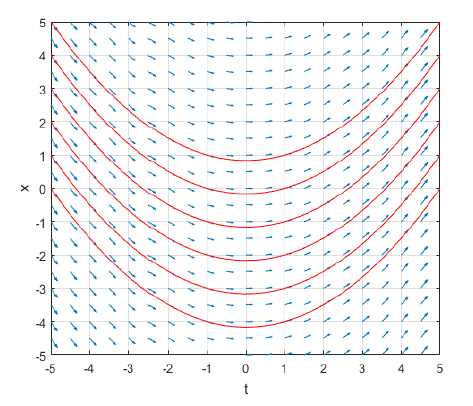
\includegraphics[width=0.8\linewidth]{UnbestimmtesIntegral.png}
      \end{center}
  \end{minipage}
  \begin{minipage}{0.45\linewidth}
    \begin{center}
      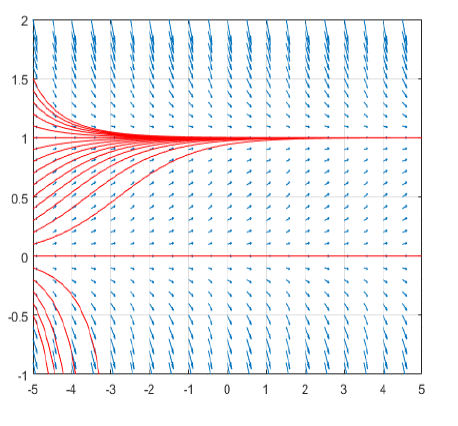
\includegraphics[width=0.9\linewidth]{AutonomeDGL.png}
      \end{center}
  \end{minipage}
\end{concept}


\begin{KR}{Richtungsfeld zeichnen und interpretieren}\\
\textbf{Steigungen} $f(x_i, y_j)$ für verschiedene Punkte $(x_i, y_j)$ berechnen

\textbf{Richtungspfeile} zeichnen: $\forall$ $(x_i, y_j)$, Steigung $f(x_i, y_j)$

\textbf{Lösungskurven:}
Von Anfangspunkt $(x_0, y_0)$ ausgehend folge Richtungspfeilen, um Lösungskurve zu approximieren.

\small
\textbf{Python-Implementierung}
Verwende \texttt{numpy.meshgrid()} und \texttt{pyplot.quiver()} zur automatischen Darstellung.
\end{KR}

\subsubsection{Numerische Lösungsverfahren}

\begin{definition}{Idee des Euler-Verfahrens}

\begin{minipage}{0.69\linewidth}
Euler-Verfahren folgt Tangente im Punkt $(x_i, y_i)$ mit Steigung $f(x_i, y_i)$ um Schrittweite $h$. 

$\rightarrow$ einfachstes Einschrittverfahren mit\\ Konvergenzordnung $p = 1$.
\end{minipage}
\begin{minipage}{0.3\linewidth}
  \begin{center}
    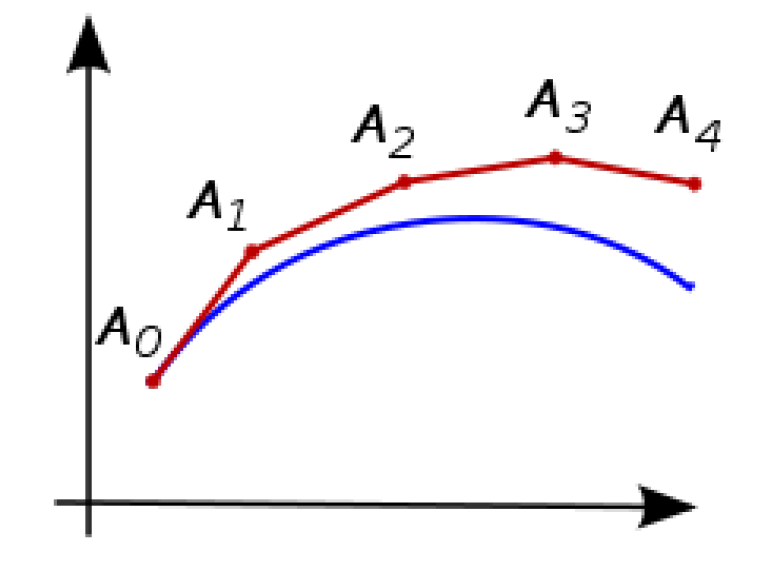
\includegraphics[width=\linewidth]{Newtonverfahren.png}
    \end{center}
\end{minipage}
\end{definition}

\begin{concept}{Eulerverfahren}
  \small
  Findet Geraden mit Steigung $f(x_i,y_i)$ für Punkte $(x_i,y_i)$
  \vspace{1mm}\\ 
  \normalsize
  \textbf{DGL} am Punkt $(x_i,y_i)$: $y'=f(x_i,y_i) \rightarrow y=y_i+f(x_i,y_i)\cdot (x-x_i)$
  \vspace{1mm}\\
  \textbf{AWP:} $y' = f(x,y)$ mit $y(a) = y_0$ auf dem Intervall $[a,b]$
  \vspace{1mm}\\
  \textbf{Euler-Verfahren} mit Schrittweite $h = \frac{b-a}{n}$:
  $$x_{i+1} = x_i + h$$
  $$y_{i+1} = y_i + h \cdot f(x_i, y_i)$$
  Gegebene Anfangswerte: $x_0 = a$, $x_i = a + ih$ für $i = 0, ..., n-1$ und $y_0$
  \small
  Problem: Steigung wird nur am linken Ende des Intervalls berücksichtigt! 
\end{concept}

\begin{theorem}{Anfangswerte berechnen} Für $i=0$ und $x=x_0$: \\
  $\underbrace{y_1}_{\approx y(x_1)}=y_0+f(x_0,y_0)\cdot\underbrace{(x_1-x_0)}_{=h}$
  $\rightarrow x_i = x_0 + i \cdot h$
\end{theorem}



\begin{KR}{Euler-Verfahren anwenden}
AWP $y' = f(x,y)$, $y(a) = y_0$, Intervall $[a,b]$

\textbf{Parameter:}
$n$ = Anzahl Schritte, berechne: $h = \frac{b-a}{n}$

\textbf{Startwerte:}
$x_0 = a$, $y_0 = $ gegebener Anfangswert

\textbf{Iteration}
für $i = 0, 1, ..., n-1$:
\begin{itemize}
    \item Berechne $f(x_i, y_i)$
    \item Setze $x_{i+1} = x_i + h$ und $y_{i+1} = y_i + h \cdot f(x_i, y_i)$
\end{itemize}
\textbf{Absoluter Fehler:}
$|y(x_n) - y_n|$ ($y(x_n)$ = exakte Lösung an Stelle $x_n$)
\vspace{1mm}\\
\small
\textbf{Interpretation:}
Punkte $(x_i, y_i)$ approximieren Lösung $y(x)$ an den Stützstellen
\end{KR}

\begin{example2}{Euler-Verfahren}
$\frac{dy}{dx} = \frac{x^2}{y}$ mit $y(0) = 2$ auf Intervall $[0, 1.4]$ 

\textbf{Parameter:} $n = 2$, $h = 0.7$

\textbf{Iteration 0:}
\begin{itemize}
    \item $i = 0$: $x_0 = 0$, $y_0 = 2 \rightarrow f(0, 2) = \frac{0^2}{2} = 0$
    \item $x_1 = 0 + 0.7 = 0.7$ und $y_1 = 2 + 0.7 \cdot 0 = 2$
\end{itemize}
\textbf{Iteration 1:}
\begin{itemize}
    \item $i = 1$: $x_1 = 0.7$, $y_1 = 2 \rightarrow f(0.7, 2) = \frac{0.7^2}{2} = 0.245$
    \item $x_2 = 0.7 + 0.7 = 1.4$ und $y_2 = 2 + 0.7 \cdot 0.245 = 2.1715$
\end{itemize}

\textbf{Exakte Lösung:} $y(x) = \sqrt{\frac{2x^3}{3} + 4}$
$y(1.4) = \sqrt{\frac{2 \cdot 1.4^3}{3} + 4} = 2.253$

\textbf{Absoluter Fehler:} $|2.253 - 2.1715| = 0.0815$
\end{example2}

\subsubsection{Verbesserte Euler-Verfahren}

\begin{theorem}{Mittelpunkt-Verfahren}
berechnet Steigung in der Mitte des Intervalls:
$$x_{h/2} = x_i + \frac{h}{2} \text{ und } y_{h/2} = y_i + \frac{h}{2} \cdot f(x_i, y_i)$$
$$x_{i+1} = x_i + h \text{ und } y_{i+1} = y_i + h \cdot f(x_{h/2}, y_{h/2})$$
\small
Konvergenzordnung: $p = 2$
\end{theorem}

\begin{corollary}{Modifiziertes Euler-Verfahren (Heun-Verfahren)}\\
verwendet den Durchschnitt zweier Steigungen:
$$k_1 = f(x_i, y_i) \text{ und } k_2 = f(x_i + h, y_i + h \cdot k_1)$$
$$x_{i+1} = x_i + h \text{ und } y_{i+1} = y_i + h \cdot \frac{k_1 + k_2}{2}$$
\small
Konvergenzordnung: $p = 2$
\end{corollary}

\begin{example2}{Vergleich der Euler-Verfahren} AWP aus vorigem Bsp\\
\textbf{Mittelpunkt-Verfahren:}
\begin{itemize}
    \item $x_{1/2} = 0.35$, $y_{1/2} = 2$, $f(0.35, 2) = 0.061$
    \item $y_1 = 2 + 0.7 \cdot 0.061 = 2.043$
    \item $x_{3/2} = 1.05$, $y_{3/2} = 2.128$, $f(1.05, 2.128) = 0.518$
    \item $y_2 = 2.043 + 0.7 \cdot 0.518 = 2.406$
\end{itemize}
\vspace{2mm}
\textbf{Modifiziertes Euler-Verfahren:}
\begin{itemize}
    \item $k_1 = 0$, $k_2 = f(0.7, 2) = 0.245$
    \item $y_1 = 2 + 0.7 \cdot \frac{0 + 0.245}{2} = 2.086$
    \item $k_1 = 0.245$, $k_2 = f(1.4, 2.257) = 0.866$
    \item $y_2 = 2.086 + 0.7 \cdot \frac{0.245 + 0.866}{2} = 2.475$
\end{itemize}
\vspace{2mm}
\textbf{Fehlervergleich bei $x = 1.4$:}
\begin{itemize}
    \item Exakt: $y(1.4) = 2.253$
    \item Euler: $|2.253 - 2.172| = 0.081$
    \item Mittelpunkt: $|2.253 - 2.406| = 0.153$
    \item Modifiziert: $|2.253 - 2.475| = 0.222$
\end{itemize}
\end{example2}

\subsubsection{Runge-Kutta Verfahren}

\begin{KR}{Runge-Kutta Verfahren}
Das klassische Runge-Kutta Verfahren verwendet vier Steigungen und hat Konvergenzordnung $p = 4$:

\textbf{Steigungen berechnen:}
\vspace{-2mm}\\
$$k_1 = f(x_i, y_i), \quad
k_2 = f(x_i + \frac{h}{2}, y_i + \frac{h}{2} k_1)$$
$$k_3 = f(x_i + \frac{h}{2}, y_i + \frac{h}{2} k_2), \quad
k_4 = f(x_i + h, y_i + h k_3)$$

\textbf{Gewichtetes Mittel bilden}:
$\text{Steigung} = \frac{1}{6}(k_1 + 2k_2 + 2k_3 + k_4)$

\textbf{Nächsten Punkt berechnen}:
$x_{i+1} = x_i + h$ und $y_{i+1} = y_i + h \cdot \text{Steigung}$

\textbf{Iteration fortsetzen}:
Wiederhole bis zum Ende des Intervalls.
\end{KR}

\begin{concept}{Butcher-Schema}
    Charakterisiert Runge-Kutta Verfahren:

    \begin{minipage}{0.45\textwidth}
        \begin{center}
        \begin{tabular}{c|cccc}
        0 & & & & \\
        $\frac{1}{2}$ & $\frac{1}{2}$ & & & \\
        $\frac{1}{2}$ & 0 & $\frac{1}{2}$ & & \\
        1 & 0 & 0 & 1 & \\
        \hline
        & $\frac{1}{6}$ & $\frac{1}{3}$ & $\frac{1}{3}$ & $\frac{1}{6}$
        \end{tabular}
        \end{center}
    \end{minipage}
    \begin{minipage}{0.54\textwidth}
        \textbf{Interpretation:} Die erste Spalte gibt die Stufen $c_i$, 
        die zweite Spalte die Koeffizienten $a_{ij}$ für die Steigungen $k_j$ und die letzte Zeile die Gewichtung der Steigungen für die nächste Iteration an.
    \end{minipage}

\end{concept}


\begin{example2}{Vergleich numerischer Verfahren}
AWP: $\frac{dy}{dx} = x + y^2, \quad y(0) = 0$
auf dem Intervall $[0, 1]$ mit Schrittweite $h = 0.2$.

\paragraph{Euler-Verfahren}
$f(x,y) = x + y^2$, $h = 0.2$, $n = 5$

\textbf{Iteration 0 $\rightarrow$ 1:}
$x_0 = 0, y_0 = 0$
$f(0, 0) = 0 + 0^2 = 0$

$x_1 = 0.2, y_1 = 0 + 0.2 \cdot 0 = 0$

\textbf{Iteration 1 $\rightarrow$ 2:}
$x_1 = 0.2, y_1 = 0$
$f(0.2, 0) = 0.2 + 0^2 = 0.2$
$x_2 = 0.4, y_2 = 0 + 0.2 \cdot 0.2 = 0.04$

usw... \textbf{Euler-Ergebnis:} $y(1) \approx 0.4150$

\paragraph{Runge-Kutta Verfahren}

\textbf{Schritt 0 $\rightarrow$ 1:} $x_0 = 0, y_0 = 0$

$k_1 = f(0, 0) = 0$,
$k_2 = f(0.1, 0) = 0.1$

$k_3 = f(0.1, 0.01) = 0.1 + 0.01^2 = 0.1001$

$k_4 = f(0.2, 0.02002) = 0.2 + 0.02002^2 = 0.2004$

$y_1 = 0 + \frac{0.2}{6}(0 + 2 \cdot 0.1 + 2 \cdot 0.1001 + 0.2004) = 0.0200$

\textbf{Schritt 1 $\rightarrow$ 2:} $x_1 = 0.2, y_1 = 0.0200$

$k_1 = f(0.2, 0.0200) = 0.2 + 0.0004 = 0.2004$

$k_2 = f(0.3, 0.0400) = 0.3 + 0.0016 = 0.3016$

$k_3 = f(0.3, 0.0502) = 0.3 + 0.0025 = 0.3025$

$k_4 = f(0.4, 0.0805) = 0.4 + 0.0065 = 0.4065$

$y_2 = 0.0200 + \frac{0.2}{6}(0.2004 + 2 \cdot 0.3016 + 2 \cdot 0.3025 + 0.4065) = 0.0801$

usw... 

\textbf{Runge-Kutta Ergebnisse:}

$y_1 = 0.0200, y_2 = 0.0801, y_3 = 0.1806, y_4 = 0.3214, y_5 = 0.5027$

\textbf{Runge-Kutta-Ergebnis:} $y(1) \approx 0.5027$

\paragraph{Genauigkeitsvergleich:}
Genaue Lösung: $y(1) \approx 0.5463$

Fehler:
\begin{itemize}
    \item Euler: $|0.5463 - 0.4150| = 0.1313$
    \item Runge-Kutta: $|0.5463 - 0.5027| = 0.0436$
\end{itemize}
Das Runge-Kutta Verfahren ist etwa 3-mal genauer.

\paragraph{Konvergenzordnung:}
\begin{itemize}
    \item Euler-Verfahren: Konvergenzordnung $p = 1$
    \item Runge-Kutta 4: Konvergenzordnung $p = 4$
\end{itemize}

Bei Halbierung der Schrittweite erwarten wir:
\begin{itemize}
    \item Euler: Fehler halbiert sich
    \item RK4: Fehler wird um Faktor 16 kleiner
\end{itemize}
\end{example2}

\raggedcolumns
\columnbreak

\subsubsection{Systeme von Differentialgleichungen}

\begin{definition}{DGL höherer Ordnung $\rightarrow$ System 1. Ordnung}\\
  \small
Jede DGL $n$-ter Ordnung kann in ein System von $n$ DGL 1. Ordnung umgewandelt werden durch Einführung von Hilfsvariablen für die Ableitungen.
\end{definition}

\begin{KR}{DGL höherer Ordnung auf System 1. Ordnung zurückführen}

\textbf{Nach höchster Ableitung auflösen}:\\
Bringe die DGL in die Form $y^{(n)} = f(x, y, y', ..., y^{(n-1)})$.
\vspace{2mm}\\
\begin{minipage}{0.4\linewidth}
\textbf{Hilfsvariablen einführen}
\small
$$z_1(x) = y(x)$$
$$z_2(x) = y'(x)$$
$$...$$
$$z_n(x) = y^{(n-1)}(x)$$
\end{minipage}
\hspace{2mm}
\begin{minipage}{0.4\linewidth}
\textbf{System aufstellen}
 \small
$$z_1' = z_2$$
$$...$$
$$z_{n-1}' = z_n$$
$$z_n' = f(x, z_1, z_2, ..., z_n)$$
\end{minipage}

\textbf{Vektorielle Schreibweise}:
$\mathbf{z}' = \mathbf{f}(x, \mathbf{z})$ mit $\mathbf{z}(x_0) = \begin{psmallmatrix} y(x_0) \\ y'(x_0) \\ \cdots \\ y^{(n-1)}(x_0) \end{psmallmatrix}$
\end{KR}

\begin{example2}{Landende Boeing - DGL 2. Ordnung}
Eine Boeing 737-200 landet mit $v_0 = 100$ m/s und erfährt die Bremskraft $F = -5\dot{x}^2 - 570000$. Die Bewegungsgleichung ist:
$mx'' = -5{x'}^2 - 570000$
mit $m = 97000$ kg. Formen Sie in ein System 1. Ordnung um.

\textbf{Nach $x''$ auflösen:}
$x'' = \frac{-5{x'}^2 - 570000}{97000}$

\textbf{Hilfsvariablen:}

$z_1(t) = x(t) = \text{ Position}$ 

$z_2(t) = x'(t) = v(t) = \text{ Geschwindigkeit}$

\textbf{System 1. Ordnung:} $z_1' = z_2$ und
$z_2' = \frac{-5z_2^2 - 570000}{97000}$

\textbf{Anfangsbedingungen:} $\mathbf{z}(0) = \begin{psmallmatrix} 0 \\ 100 \end{psmallmatrix}$

Das System kann nun mit Runge-Kutta gelöst werden.
\end{example2}

\begin{example2}{Kombinierte Anwendung mit Ausgleichsrechnung}\\
Umsatzentwicklung modelliert durch DGL:
$\frac{dU}{dt} = 0.1U(100 - U) - S(t)$

$U(t)$ = Umsatz in Millionen €, $S(t) = 20\sin(2\pi t)$ = saisonale Schwankungen

\textbf{Klassifikation:}
\begin{itemize}
    \item Nichtlineare DGL 1. Ordnung (wegen $U(100-U)$ Term)
    \item Zeitabhängiger Störterm $S(t)$
\end{itemize}

\textbf{Gleichgewichtspunkte für $S = 0$:}
$\frac{dU}{dt} = 0.1U(100 - U) = 0$

Lösungen: $U^* = 0$ oder $U^* = 100$

Stabilität:
$\frac{d}{dU}(0.1U(100-U)) = 0.1(100 - 2U)$

\begin{itemize}
    \item Bei $U^* = 0$: $\frac{df}{dU} = 10 > 0 \rightarrow$ instabil
    \item Bei $U^* = 100$: $\frac{df}{dU} = -10 < 0 \rightarrow$ stabil
\end{itemize}

\begin{minipage}{0.59\linewidth}
\textbf{Numerische Lösung:}

Mit Runge-Kutta ($h = 0.1$):

System: 

$\frac{dU}{dt} = 0.1U(100-U) - 20\sin(2\pi t)$

$\frac{dS}{dt} = 20\cos(2\pi t)$
\vspace{2mm}\\
Typische Ergebnisse (Tabelle):
\end{minipage}
\begin{minipage}{0.4\linewidth}
\begin{center}
\begin{tabular}{|c|c|c|c|}
\hline
$t$ & $U(t)$ & $S(t)$ & $\frac{dU}{dt}$ \\
\hline
0 & 30.0 & 0 & 210.0 \\
1 & 45.2 & 0 & 247.6 \\
2 & 62.8 & 0 & 233.9 \\
3 & 76.1 & 0 & 182.0 \\
4 & 85.3 & 0 & 125.4 \\
5 & 91.1 & 0 & 81.2 \\
\hline
\end{tabular}
\end{center}
\end{minipage}

\textbf{Ausgleichsrechnung:} Fitten der numerischen Daten 

mit logistischer Funktion: $U(t) = \frac{K}{1 + Ae^{-rt}}$

Linearisierung durch: $\ln(\frac{K-U}{U}) = \ln(A) - rt$

Nach linearer Regression: $K \approx 100$, $A \approx 2.33$, $r \approx 0.693$

Güte des Fits: $R^2 > 0.98$

(sehr gute Anpassung an ungestörtes Wachstum)
\end{example2} 

\raggedcolumns
\columnbreak

\subsubsection{Stabilität}

\begin{remark}
  Bei der numerischen Lösung von DGL kann es vorkommen, dass der numerische Fehler unbeschränkt wächst. Dies führt zu \textbf{instabilen} Lösungen.
  \textbf{Tipp:} beginne mit einer kleinen Schrittweite und prüfe die Stabilität der Lösung.
\end{remark}

\begin{definition}{Stabilitätsfunktion}\\
Für DGL $y' = -\alpha y$ (mit $\alpha > 0$) kann die numerische Lösung in der Form
$y_{i+1} = g(h\alpha) \cdot y_i$
geschrieben werden. 

Die Funktion $g(z)$ heißt \textbf{Stabilitätsfunktion} des Verfahrens.

Das offene Intervall $z \in (0, \alpha)$, in dem $|g(z)| < 1$ gilt, bezeichnet man als \textbf{Stabilitätsintervall}.
\end{definition}

\begin{example2}{Stabilität des Euler-Verfahrens} $y' = -2.5y$ mit $y(0) = 1$.

\textbf{Euler-Verfahren:} $y_{i+1} = y_i - h \cdot 2.5 y_i = y_i(1 - 2.5h)$

\textbf{Stabilitätsfunktion:} $g(z) = 1 - z$ mit $z = 2.5h$

\textbf{Stabilitätsbedingung:} $|1 - 2.5h| < 1$
$\Rightarrow 0 < 2.5h < 2 \Rightarrow 0 < h < 0.8$

\textbf{Verhalten:}
\begin{itemize}
    \item $h = 0.2$: Stabile Lösung (exponentieller Abfall)
    \item $h = 0.85$: Instabile Lösung (Oszillation mit wachsender Amplitude)
\end{itemize}

\textbf{Exakte Lösung:} $y(x) = e^{-2.5x}$ (streng monoton fallend)
\end{example2}

\subsubsection{Fehlerordnung und Konvergenz}

\begin{definition}{Lokaler und globaler Fehler}\\
\textbf{Lokaler Fehler:} Fehler nach einer Iteration
$\varphi(x_i, h) := y(x_{i+1}) - y_{i+1}$

\textbf{Globaler Fehler:} Der Fehler nach $n$ Iterationen
$y(x_n) - y_n$

\textbf{Konsistenzordnung $p$:} \\ Ein Verfahren hat Konsistenzordnung $p$, falls
$|\varphi(x_i, h)| \leq C \cdot h^{p+1}$

\textbf{Konvergenzordnung $p$:} \\ Ein Verfahren hat Konvergenzordnung $p$, falls
$|y(x_n) - y_n| \leq C \cdot h^p$
\end{definition}

\begin{concept}{Konvergenzordnungen der Verfahren}
\begin{itemize}
    \item \textbf{Euler-Verfahren:} Konvergenzordnung $p = 1$
    \item \textbf{Mittelpunkt-Verfahren:} Konvergenzordnung $p = 2$
    \item \textbf{Modifiziertes Euler-Verfahren:} Konvergenzordnung $p = 2$
    \item \textbf{Klassisches Runge-Kutta:} Konvergenzordnung $p = 4$
\end{itemize}

\textbf{Praktische Bedeutung:} Bei Halbierung der Schrittweite $h$ reduziert sich der Fehler um den Faktor $2^p$.
\end{concept}

\begin{example}
Konvergenzverhalten für $\frac{dy}{dx} = \frac{x^2}{y}$ mit $y(0) = 2$ auf $[0, 10]$

\textbf{Exakte Lösung:} $y(x) = \sqrt{\frac{2x^3}{3} + 4}$

\textbf{Fehler bei $x = 10$ für verschiedene $h$:}

\begin{center}
\begin{tabular}{|c|c|c|c|c|}
\hline
$h$ & Euler & Mittelpunkt & Mod. Euler & Runge-Kutta \\
\hline
0.1 & $10^{-1}$ & $10^{-2}$ & $10^{-2}$ & $10^{-5}$ \\
\hline
0.05 & $5 \times 10^{-2}$ & $2.5 \times 10^{-3}$ & $2.5 \times 10^{-3}$ & $6 \times 10^{-7}$ \\
\hline
0.025 & $2.5 \times 10^{-2}$ & $6 \times 10^{-4}$ & $6 \times 10^{-4}$ & $4 \times 10^{-8}$ \\
\hline
\end{tabular}
\end{center}

\textbf{Beobachtung:} Bei Halbierung von $h$:
\begin{itemize}
    \item Euler: Fehler halbiert sich (Ordnung 1)
    \item Mittelpunkt/Mod. Euler: Fehler viertelt sich (Ordnung 2)
    \item Runge-Kutta: Fehler wird um Faktor 16 kleiner (Ordnung 4)
\end{itemize}
\end{example}

\begin{KR}{Wann welches Verfahren?}
\begin{itemize}
    \item \textbf{Euler:} Einfachste Implementierung, Lernzwecke, grobe Näherungen
    \item \textbf{Mittelpunkt/Modifiziert:} \\Bessere Genauigkeit als Euler, moderater Aufwand
    \item \textbf{Runge-Kutta 4:} Standard für die meisten Probleme, gute Balance zwischen Genauigkeit und Aufwand
\end{itemize}
\end{KR}






